%%%%%%%%%%%%%%%%%%%%%%%%%%%%%%%%%%%%%%%%%%%%%%%%%%%%%%%%%%%%%%%%%%% 
%                                                                 %
%                            CHAPTER SIX                          %
%                                                                 %
%%%%%%%%%%%%%%%%%%%%%%%%%%%%%%%%%%%%%%%%%%%%%%%%%%%%%%%%%%%%%%%%%%% 
 





\chapter{EXPERIMENTS AND RESULTS} \label{sec:results}
Suppose we are given a social network with signs, but a
small fraction of the edge signs are ``hidden''. How can we predict
these signs with the information provided by the rest of network? In this chapter, we study the {\it edge sign prediction
  problem} using online social network data. The prediction algorithm in this work is a direct implementation of the convergence model. Our experimental results match and surpass the state of art. The results provide empirical support of the convergence model, as well as the extended balance theory behind it.

We justify that the convergence model is able to predict these ``hidden'' signs from the theoretical aspect. Let's
denote the original social network with all signed edges as $G$, the
network consisting of hidden edges as $G_{h}$, and the network
consisting of the remaining edges as $G_{r}$. The edges (relations)
between each pair of nodes is measured by $\{+,\,-,\,O\}$. We run the
convergence model on $G_{r}$, and denote the network after convergence
as $G_{r}^{'}$. We expect that the signs of the hidden edges in
$G_{r}^{'}$ largely agree with the true signs.

By the assumption that every social network has a tendency towards
balance, it can be inferred that $G$ is largely balanced at any
moment. Hence, the majority of $G_{r}$ is balanced. The only
exceptions are the components with hidden edges, which are of sign $O$
in $G_{r}$. By the principle of total relation cost minimization, the
changes mostly occur on the $O$-sign hidden edges during the
convergence. We expect the hidden edges in $G_h$ to have their
true signs in $G_{r}^{'}$ if $G$ is largely balanced.

We compare our algorithm to force directed algorithm (FD)
in~\cite{golbeck:distrust2011}. Note that we have tuned our
implementation of FD to provide similar performance reported in this
work. Even though this work combines two algorithms, in our comparison
experiments, we find that FD alone gives equally good prediction
performance on all three datasets as the combination. Despite its more
global nature, the second algorithm (PP)
from~\cite{golbeck:distrust2011} does not contribute to significant performance gains. 
\section{Data and Algorithm}
We use the same three datasets as it is
in~\cite{Leskovec:2010},~\cite{golbeck:distrust2011} to conduct our
experiments, all provided by the Stanford Large Network Dataset
Collection.
\begin{itemize}
\item Epinions is a product review website where users give reviews
  and ratings on product articles. Users can choose to trust or
  distrust others. The network contains more than $100,000$ users and
  over $700,000$ trust/distrust edges.
\item Slashdot is a technology news website where users rate each
  other as friends or foes. The dataset released in February 2009
  contains over $77,000$ users and over $900,000$ friend/foe edges.
\item Wikipedia elections collects the votes by Wikipedia users in
  elections for promoting candidates as administrators. Each user can
  give a supporting (positive) or opposing (negative) vote on the
  promotion of another. The dataset has about $7,000$ users and around
  $100,000$ votes(edges).
\end{itemize}

All edges are treated as undirected in our experiments. Due to both
the memory and computational cost of SM, running SM on the entire
dataset is infeasible. As a result, we generate random samples of our
datasets using the snowball sampling method in which a small number of
seeds with degree greater than a given threshold $deg$ are selected at
random, then all nodes that are adjacent to the seed node are selected
iteratively until the desired network size is reached.
%% Observe the fact that the influence on the
%% relation between two nodes is generated within their
%% ``community". Hence, for each hidden edge, we can confidently make the
%% prediction without referring to the edges outside its ``community". We
%% generate sub-networks with limited size as such ``communities" by the
%% following manner.
%% \begin{verbatim}
%% generate_Community(M, k, deg, G)
%%     1. pick up k random nodes whose degree>deg from G
%%     2. Create a subgraph G' with the k nodes and 0 edges
%%     3. If (size of G')<M
%%            For each u that is adjacent to some v in G':
%%                add u to G'
%%                add edges (w, u) for all w in G'
%%     4. return G'
%% \end{verbatim}
%% $G^{'}$ returned by the above function is the sub-network consisting
%% of the ``communities" of $k$ random nodes that have relatively large
%% degrees. The average size of each ``community" is therefore $M/k$.
In our practice, the size of the resulting graph is in the range
$3,000-5,000$ nodes, $k$ is chosen from $2-10$ randomly and $deg$ is
chosen from $7-20$ randomly. For each dataset, we generate 10 such
sub-networks and run tests through 10-fold cross validation. The
number of edges in a sub-network of Epinions is around $180,000$, the
number of $Slashdot$ is around $65,000$ and the number of Wikipedia
votes is around $160,000$. In the implementation of SM, the
partitioning of the distance domain satisfies $b_{+} < 1/2b_{-}$,
conforming to our theory. The weight of each type of edge satisfies
$w_{O}<<w_{+}<1/2w_{-}$. The first inequality has been argued in
previous section. The second one is chosen empirically, indicating
that a negative edge has larger influence than a positive one. Note
that we use the same setting for all the networks and do not employ
any other adjustable parameters.
\begin{algorithm}
 \KwData{$M, k, deg, G$}
 \KwResult{$Pt, Nt$}
 Get $G'=$ generate-subgraph$(M, k, deg, G)$\;
 Partition $G'$ into 10 groups of test and training samples\;
 Create two empty sets $Pt$, $Nt$\;
 \For{each of the groups}{
 run SM on the training sample and get the layout\;
 \For{each edge e in the testing sample}{
 compute its distance in the layout\;
 \eIf{e is a positive edge}{
   add its distance to $Pt$\;
   }{
   add its distance to $Nt$\;
  }
 }
 }
 \caption{SM Prediction}
\end{algorithm}

\section{Results}
The distances of testing edges are computed by the
layout of the training data. Given a distance threshold, the sign of
each edge is predicted as positive if and only if its distance is
smaller than the threshold. In the previous work, such threshold is
computed from the (distance,sign) pairs of the training samples using
standard machine learning
techniques~\cite{Leskovec:2010},~\cite{golbeck:distrust2011}. In this
thesis, however, we do not concentrate on the learning process. The
issue of interest is how good the convergence model performs in
separating hidden positive edges from negative ones in terms of
distance. Instead of making predictions based on particular threshold,
we draw ROC curves for evaluation. We consider different distance
thresholds and compute the false and trust positive rates based on the
computed $Pt$ ($Nt$) values returned by the SM Prediction Algorithm. The ROC curves in Figure~\ref{fig:ROC} are drawn upon the
$Pt$ ($Nt$) values from the accumulation of all testing samples.
\begin{figure}[th]
\centering
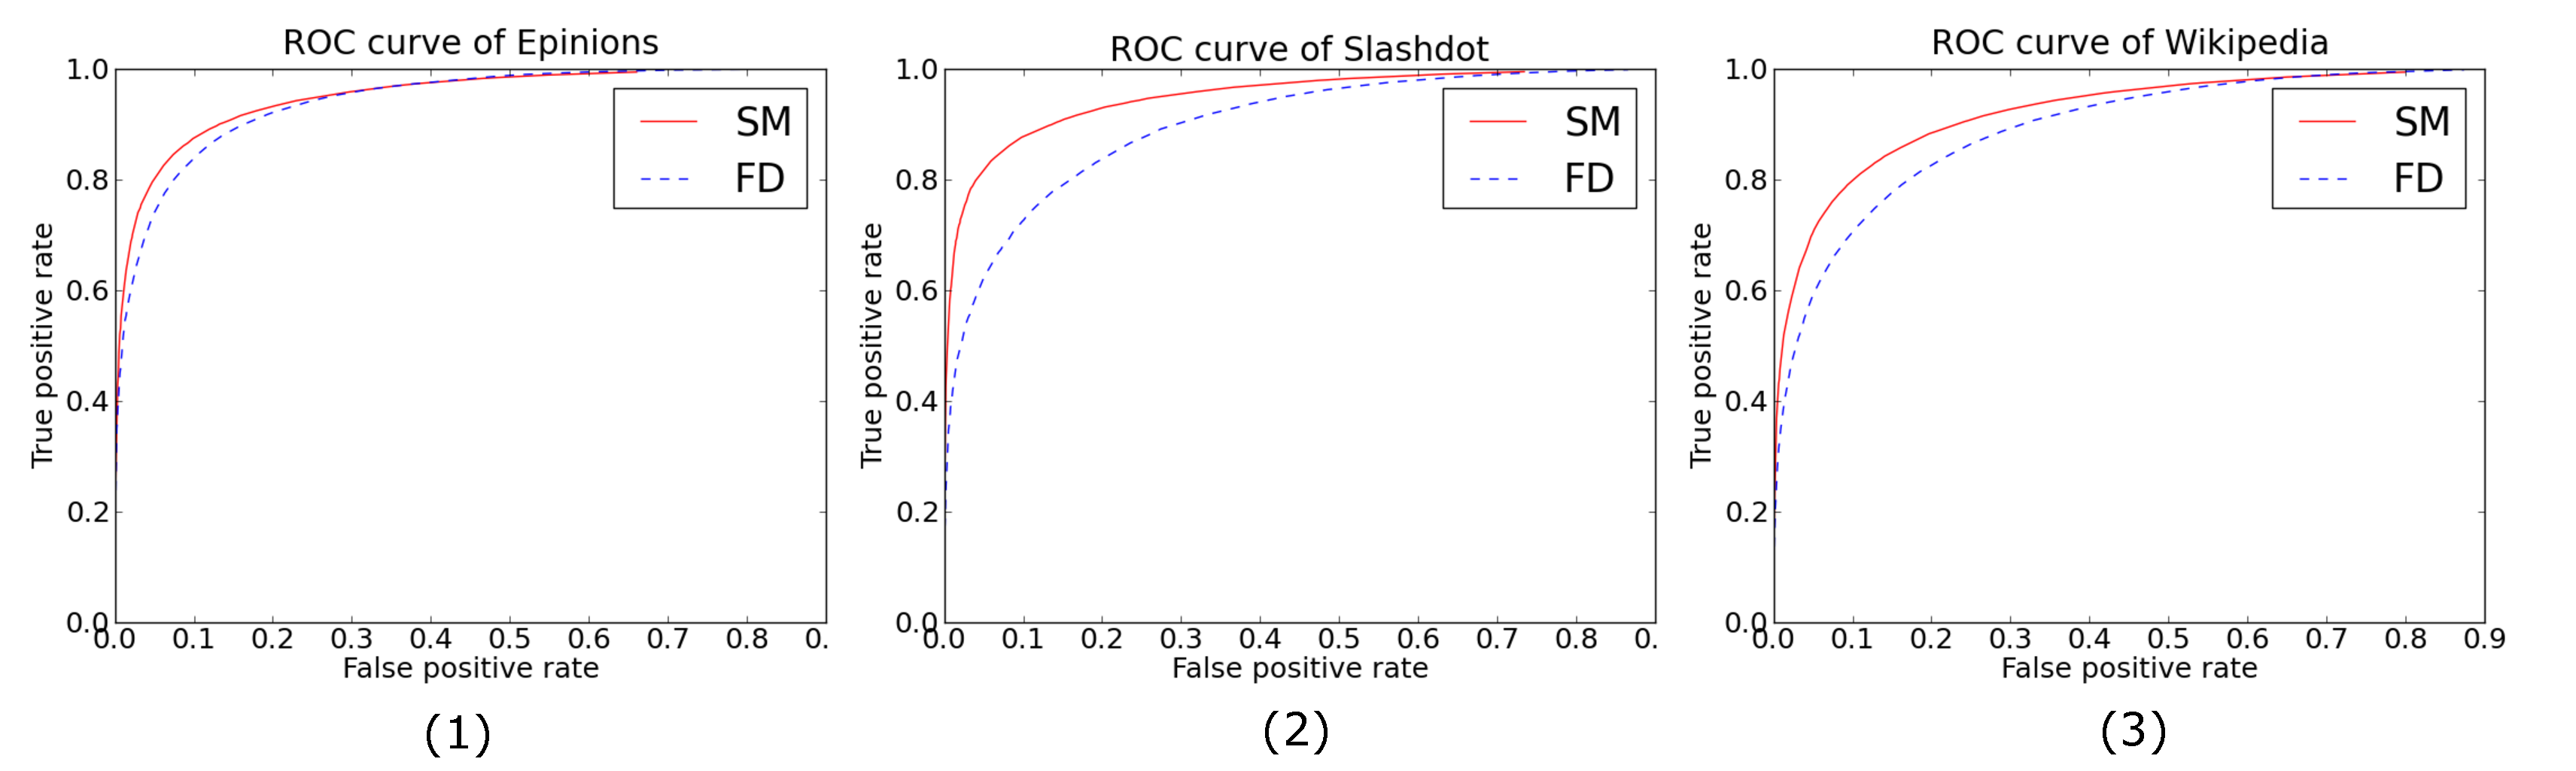
\includegraphics[height=1.8in]{Figs/ROC_curve.pdf}
\caption{\label{fig:ROC}The ROC curves are drawn upon
  distances of hidden edges, generated by SM and FD. (1) (2) (3)
  correspond to the ROC curves generated from Epinions, Slashdot and
  Wikipedia datasets respectively.}
\end{figure}

For all three datasets, we find the ROC curve of $SM$ is on the
``northwest'' side of the one of $FD$, which indicates SM is
consistently better than FD in separating hidden positive edges from
negative ones. Notice that the improvement for Slashdot is the most
significant one among the three. The possible explanation is in
Slashdot edges represent ``friends'' or ``foes'', which is by nature a
more clear identification of trust and distrust, whereas in votes in
Wikipedia or distrusting reviews of other users in Epinions are not as
strong distrust relations.  As a result, our convergence model
characterizes its mutual relation based structure nicely, and hence
produces good prediction performance.

On the Epinions and Slashdot datasets, the best thresholds on ROC
curve give $88-90 \%$ accuracy on both positive and negative
hidden edges. For Wikipedia, we achieves $83-85 \%$ at the best
threshold. The accuracy rates of Epinions and Wikipidea match the best
results from previous work, and the one of slashdot appears to be the
best so far.
\section{General Edge Prediction}
The {\it edge sign prediction} only
deals with the existing signed edges. In predicting the sign of a
hidden edge, we already know that the edge exists in the original
network. A more general problem is to predict whether there is positive edge between arbitrary pair of nodes~\cite{Kleinberg:03}. In theory, our convergence model should
be able to make such general predictions. The difference is that we do
not know if there is a hidden edge or not. We generate the distances of
testing edges as before. Now, instead of classifying the hidden edges
in $G_{r^{'}}$ as positive/negative, we need to classify them as positive or not.

The {\it general edge prediction}, deciding whether an positive edge exists or
not, is obviously a harder problem than {\it edge signed
  prediction}. Social networks are usually sparse, and hence there are
a lot more neutral relations than biased relations. If larger
distances represent more negativeness (less positiveness), then the
distance of a neutral relation should be smaller than a negative one
and larger than a positive one. As a consequence, the distribution of
neutral edges in terms of distance should concentrate in the middle
range distances. We next study this distribution, as a preliminary
step to solve the {\it general edge prediction} problem.

For each dataset, we generate samples based on random source nodes as
before, except that we exclude the edges between the $k$ source
nodes. Instead of cross validation, we use the entire sub-network for
training, and use the $k(k-1)/2$ edges between the $k$ source nodes as
testing data, whose signs are available in the original dataset
(positive, negative or neutral, i.e. no link). Similarly, the signs of
the testing edges should not be influenced strongly by the other edges
in the network. Hence, after convergence they should get to the
distances corresponding to their true signs. We repeat the experiments
50 times over all three datasets, and collect the distances for only
the neutral testing edges.
\begin{figure}[th]
\centering
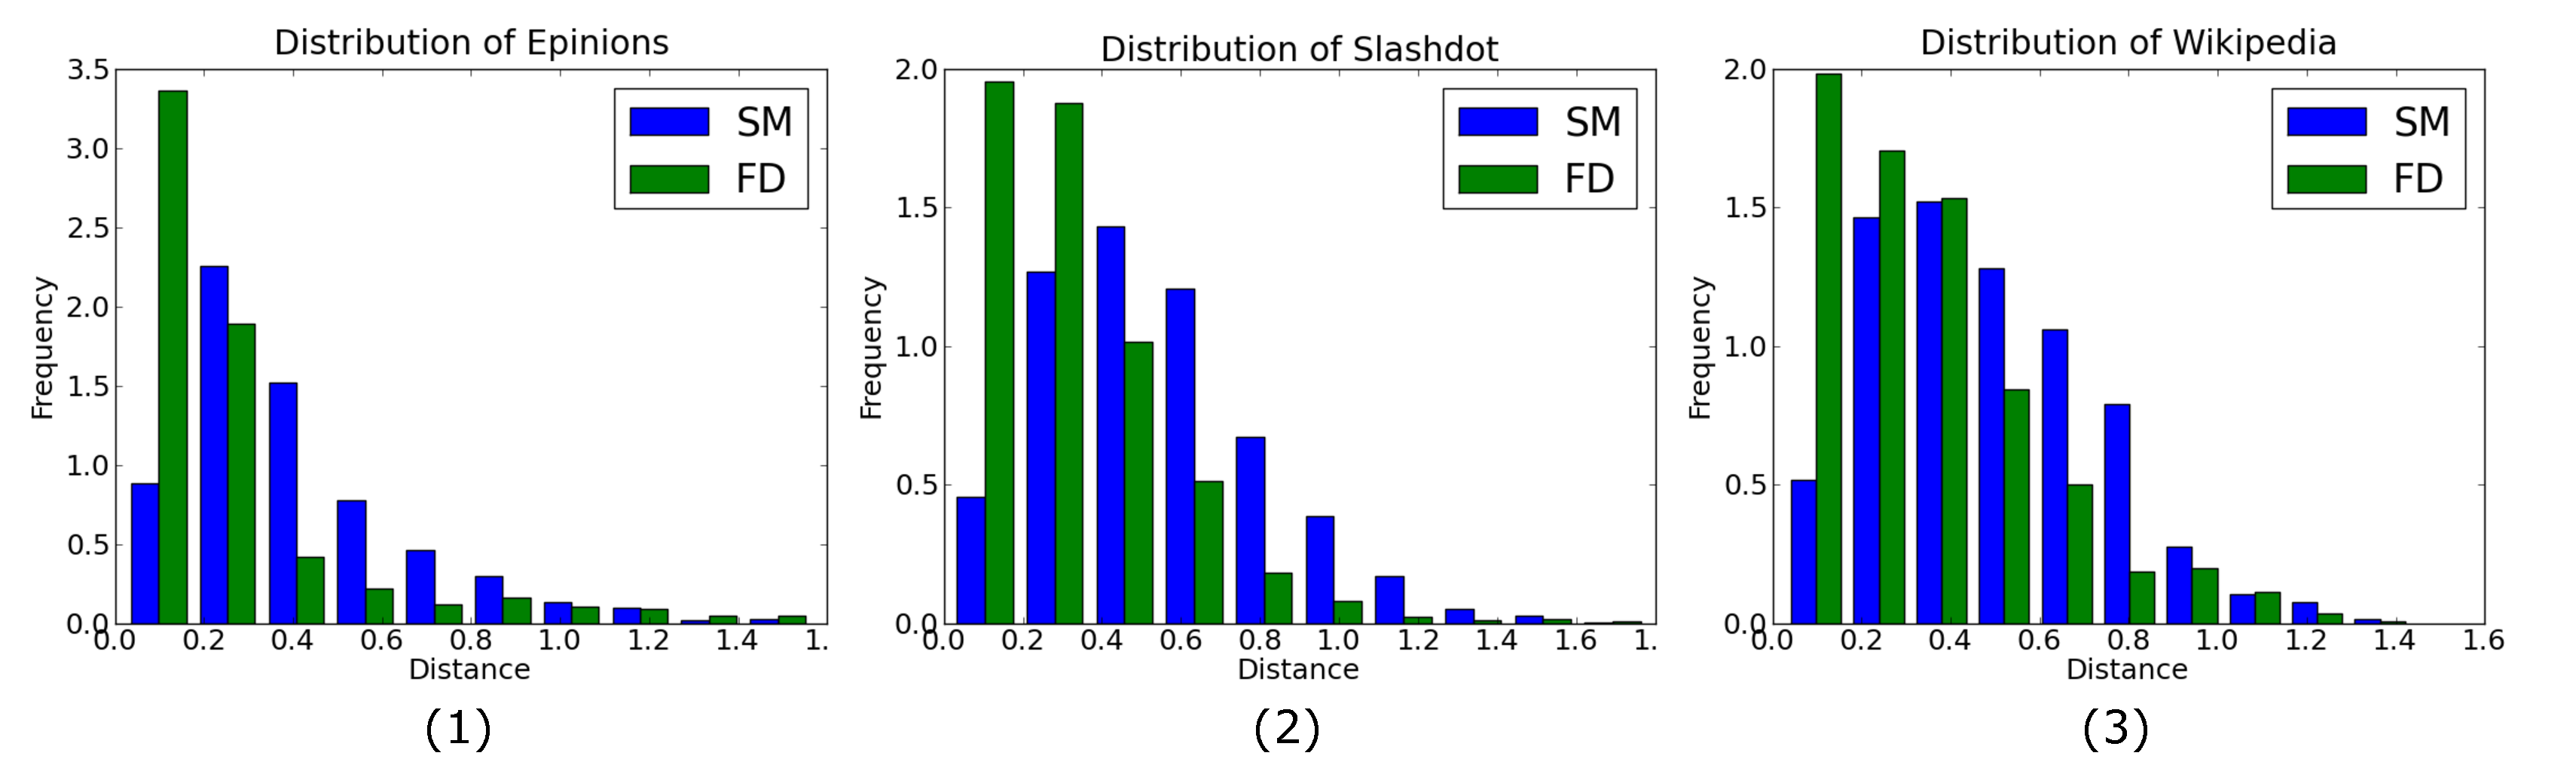
\includegraphics[height=1.8in]{Figs/hist1.pdf}
\caption{\label{hist}The histograms are drawn upon distances of
  neutral testing edges, generated by SM and FD. (1) (2) (3)
  correspond to the histograms generated from Epinions, Slashdot and
  Wikipedia datasets respectively.}
\end{figure}

As it is shown in Figure~\ref{hist}, the distances of neutral testing
edges generated by SM do relatively concentrate in the middle-range of
values following an almost Gaussian distribution. On the contrast, the
majority of neutral testing edges's distances by FD have small values,
implying a positive prediction. In fact, based on the distributions,
we can conclude that it is much more probable to classify a missing
link as a positive edge in FD than in SM.  However, SM provides more
flexibility as the distances are distributed over a larger range with
an almost Gaussian distribution, allowing us to test different tunable
algorithms.

The experimental results show the superiority of our convergence model
in predicting signed edges. Moreover, they justify that our general
balance theory is a relatively accurate description of the stable
state of social networks, and that the convergence model correctly
characterizes the dynamics of social network. As a result, our model
is a good starting point for developing algorithms for solving the
{\it general edge prediction} problem.

